\chapter{Metodología}
La metodología que usaremos para desarrollar el proyecto y mantener un seguimiento de las tareas será Scrum \cite {scrum}. Esta metodología ágil permitirá que nos adaptemos a los posibles contratiempos que se nos presenten manteniendo la efectividad y la eficiencia. 

De forma básica, como podemos observar en la figura \ref {fig:scrum_esquema}, Scrum consiste en la realización de sprints donde se consideran un grupo de tareas a realizar que aporten valor al proyecto. Al inicio de cada sprint se decidirá cuáles tareas se realizarán en este y se añadirán al \emph{Sprint Backlog}. Toda la gestión de las tareas se realizará usando la metodología Kanban que explicaremos posteriormente. Scrum recomienda realizar reuniones diarias, pero esto no será posible por la apretada agenda de los roles que forman el proyecto, por lo tanto serán substituidas por reuniones semanales. Estas reuniones podrán ser de forma presencial o telemática vía Google Meet. Al final de cada sprint se realizará una revisión de las tareas realizadas y del incremento que se ha aportado al proyecto.

\begin{figure}[h]
    \centering
    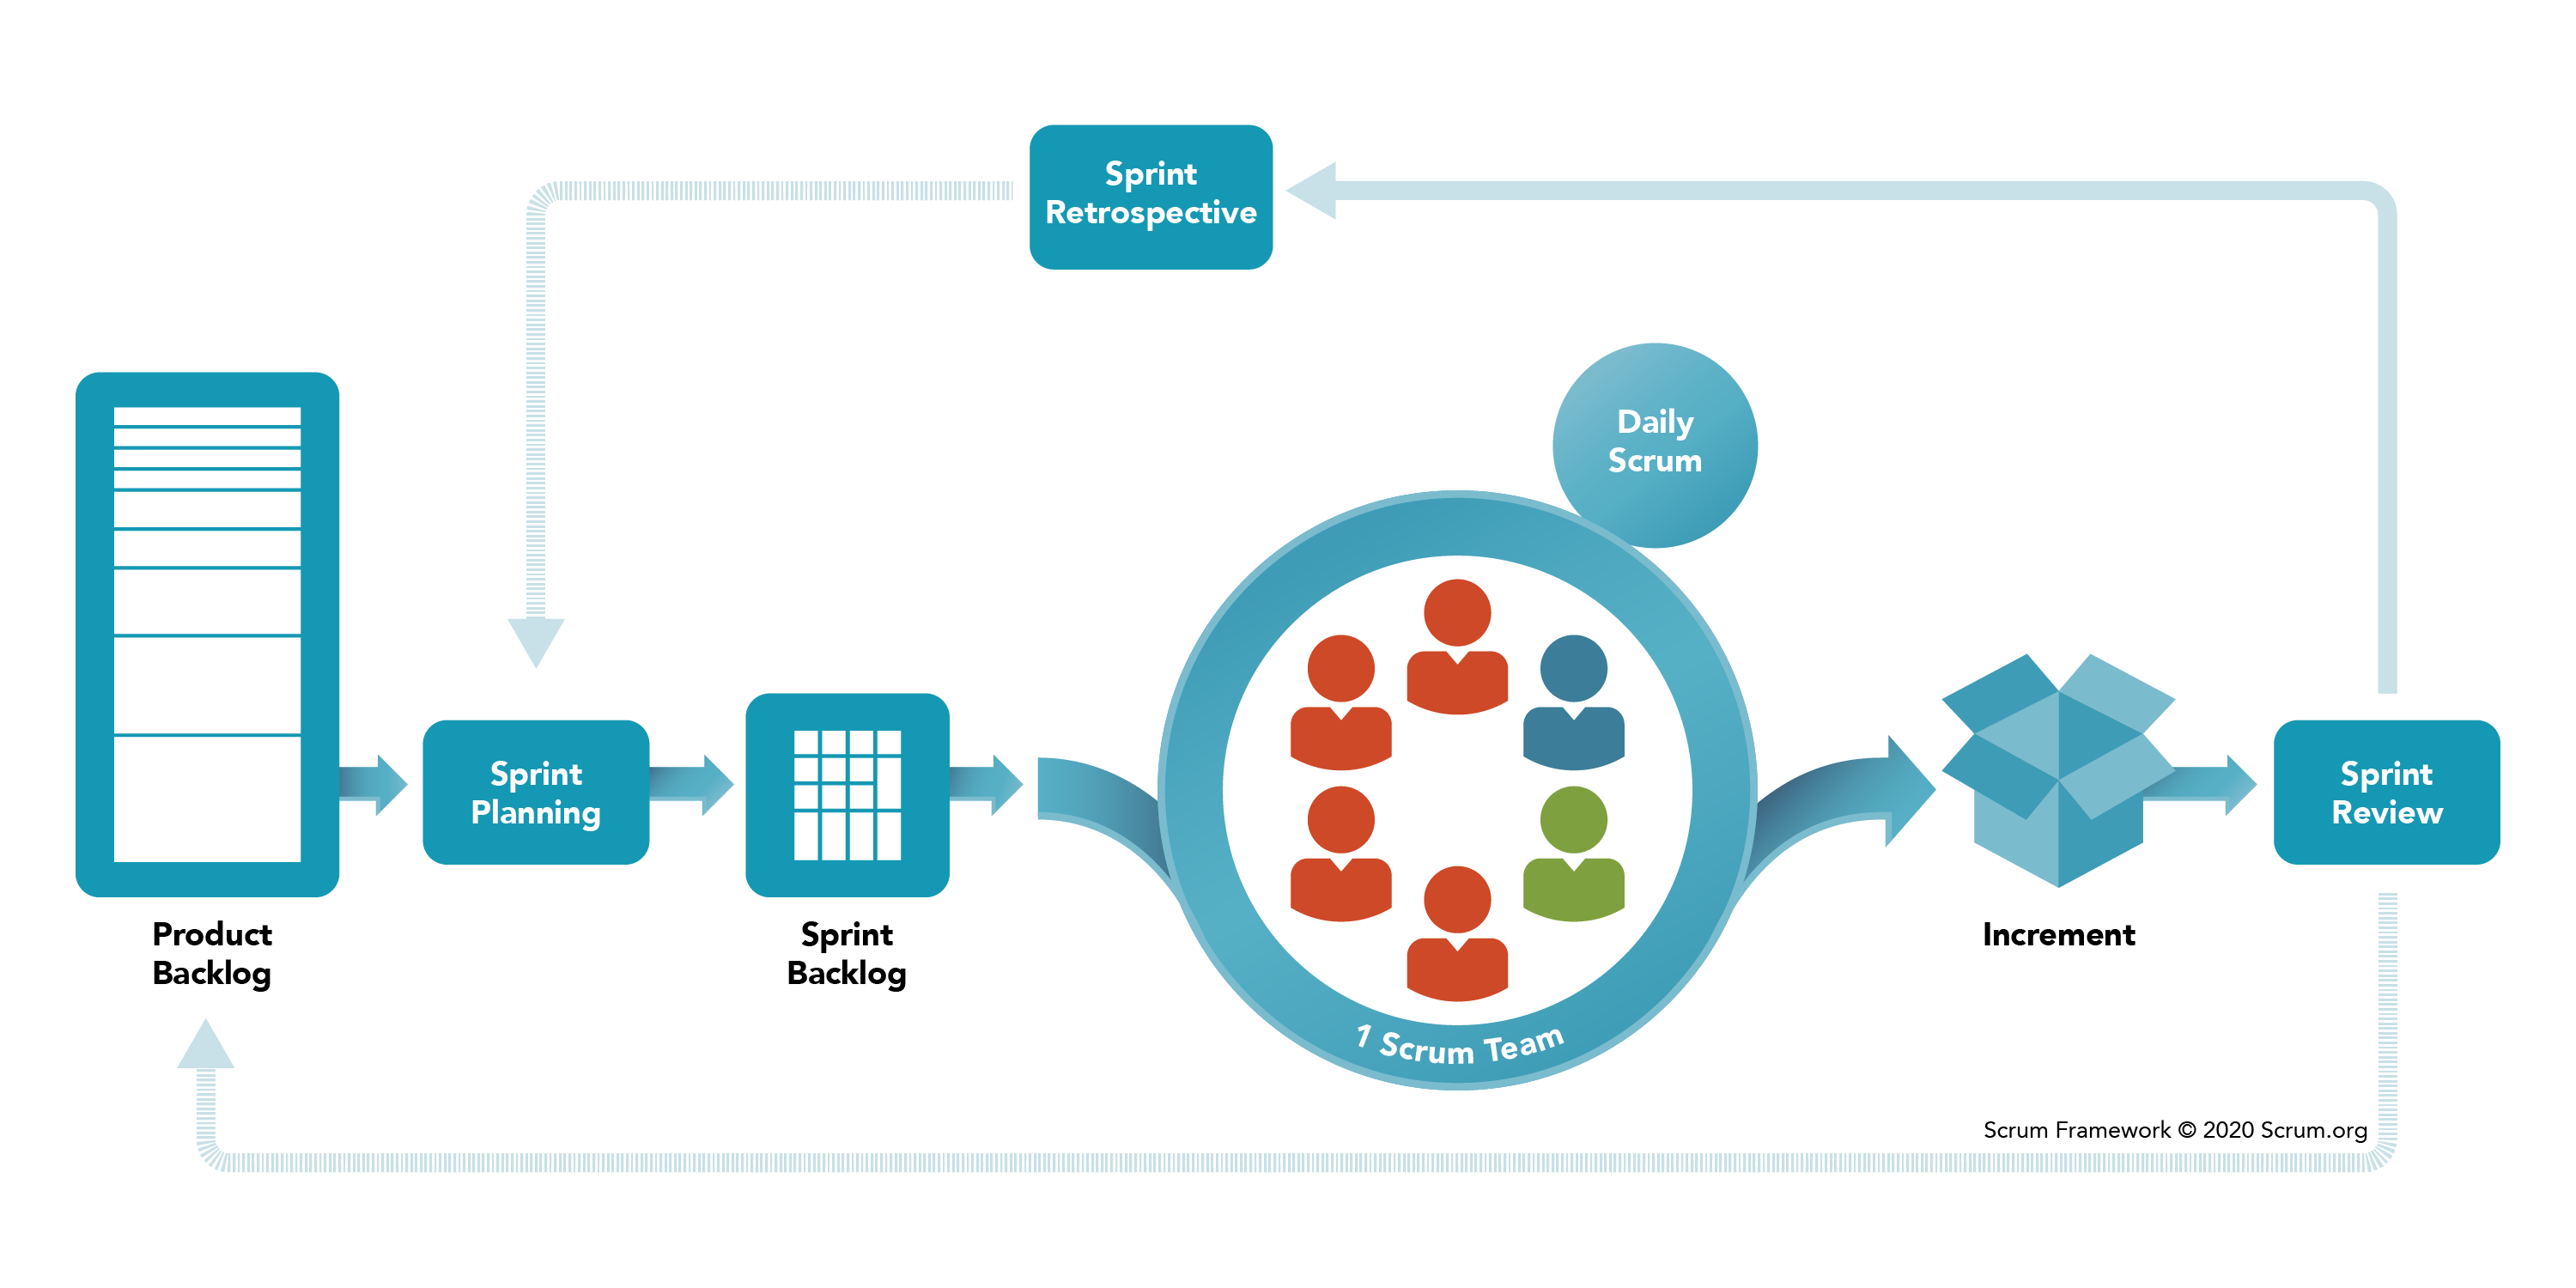
\includegraphics[width=1\textwidth]{img/scrum.png}
    \caption{Esquema básico del funcionamiento de Scrum \cite{scrum}}
    \label{fig:scrum_esquema}
\end{figure}

Para llevar un seguimiento de las tareas, usaremos la metodología Kanban, que se complementa a la perfección con la forma de llevar las tareas de Scrum. El principal objetivo de este método es manejar de forma general la forma en la que las tareas transcurren por su ciclo de vida. 

La palabra Kanban tiene un origen Japones que significa cartas visuales, donde Kan significa visual y Ban corresponde a carta. Por su etimología podemos intuir cómo funciona. Cada tarea o subtarea corresponde a una carta. Estas cartas estarán colocadas en 4 columnas diferentes:

\begin{itemize}
    \item \textbf{To Do}: Consiste en todas las tareas que son necesarias, pero que aún no se han empezado.
    \item \textbf{Doing}: Consiste en las tareas que se están desarrollando. Es importante notar que es posible que haya diversas tareas en esta columna, solo que por dependencias temporales, alguna haya quedado pausada temporalmente.
    \item \textbf{Testing}: Consiste en todas las tareas que ya se han desarrollado, pero aún no se ha comprobado su buen funcionamiento. Como es natural, no todas las tareas necesitan una fase de testeo, algunas, las más simples, se saltarán esta fase.
    \item \textbf{Completed}: Consiste en todas las tareas completadas. Esta columna es muy importante, puesto que nos basaremos principalmente en ella para observar como transcurre la planificación temporal.  
\end{itemize}
Para implementar esta metodología, usaremos la herramienta Trello, ya que se adapta a la perfección a su definición. Además tiene la ventaja  de que el director del proyecto tendrá acceso remoto y podrá hacer seguimiento inmediato de las tareas. Es importante observar que esta metodología no tiene en cuenta posibles dependencias entre tareas. Para eso, será necesario basarnos en el diagrama de Gantt que realizaremos en próximas entregas.

\section{Herramientas}
Las herramientas que usaremos para facilitar el trabajo del proyecto son las siguientes:
\begin{itemize}
    \item \textbf{LATEX}: para escribir la memoria y la documentación necesaria. Aunque es una tecnología desconocida para el autor del proyecto, a la larga facilitará el proceso de escritura.
    \item \textbf{Trello}: Para implementar la metodología antes explicada. Otra gran ventaja es la capacidad de compartir tableros. De esta manera el director del proyecto podrá realizar un seguimiento de las tareas de manera remota y añadir valoraciones para cada tarea.
    \item \textbf{Git y Gitlab de HPAI}: Al formar parte del grupo de investigación del director del proyecto, tendremos acceso, en caso de necesitarlo, a una mayor capacidad de cómputo y la ejecución se simplificará.
\end{itemize}

\section{Rigor}
Para comprobar que se cumplen los objetivos propuestos, dispondremos de varios métodos además de la ayuda proporcionada por el director y subdirector del proyecto. Puesto que es muy probable que surjan nuevas tareas durante la ejecución del proyecto, solo mencionaremos las estrategias de validación más importantes. 

Para el objetivo final, hemos de comprobar que el entorno es capaz de entrenar agentes, es por ello que entrenaremos uno como modelo de referencia. No debemos de preocuparnos de que este modelo sea eficiente, puesto que no es el objetivo del proyecto. Para elegir un buen entorno base, crearemos unas métricas cualitativas que nos sirvan para comparar los diferentes entornos y elegir el más conveniente. En la exploración del estado del arte, gracias a la experiencia del director y subdirector del proyecto, podemos estar seguros de haber cubierto una gran parte de las alternativas disponibles. Y finalmente para mantener un seguimiento de todo el proyecto, se realizarán reuniones semanales aparte de la habitual correspondencia por correo.

 
 